\documentclass[10pt]{article}
\usepackage{fullpage}
\usepackage{epsf}
\usepackage{../pplmanual}
\NeedsTeXFormat{LaTeX2e}
\typeout{^^J^^J
Parallel Programming Laboratory^^J
Manual Style^^J
Written by Milind A. Bhandarkar, 12/00^^J}

%%% Make it possible for both ps and pdf to be generated
\newif\ifpdf
\ifx\pdfoutput\undefined
  \pdffalse
\else
  \pdfoutput=1
  \pdftrue
\fi

\ifpdf
  \pdfcompresslevel=9
\fi

%%% Imported from fullpage.sty, since it is not always available
\topmargin 0pt
\advance \topmargin by -\headheight
\advance \topmargin by -\headsep

\textheight 8.9in

\oddsidemargin 0pt
\evensidemargin \oddsidemargin
\marginparwidth 1.0in

\textwidth 6.5in
%%% end import from fullpage

%%% Commonly Needed packages
\usepackage{graphicx,color,calc}
\usepackage{makeidx}
\usepackage{alltt}

%%% Commands for uniform looks of C++, Charm++, and Projections
\newcommand{\CC}{C\kern -0.0em\raise 0.5ex\hbox{\normalsize++}}
\newcommand{\emCC}{C\kern -0.0em\raise 0.4ex\hbox{\normalsize\em++}}
\newcommand{\charmpp}{\sc Charm++}
\newcommand{\projections}{\sc Projections}
\newcommand{\converse}{\sc Converse}
\newcommand{\ampi}{\sc AMPI}

%%% Commands to produce margin symbols
\newcommand{\new}{\marginpar{\fbox{\bf$\mathcal{NEW}$}}}
\newcommand{\important}{\marginpar{\fbox{\bf\Huge !}}}
\newcommand{\experimental}{\marginpar{\fbox{\bf\Huge $\beta$}}}

%%% Commands for manual elements
\newcommand{\zap}[1]{ }
\newcommand{\function}[1]{{\noindent{\textsf{#1}}\\}}
\newcommand{\cmd}[1]{{\noindent{\textsf{#1}}\\}}
\newcommand{\args}[1]{\hspace*{2em}{\texttt{#1}}\\}
\newcommand{\param}[1]{{\texttt{#1}}}
\newcommand{\kw}[1]{{\textsf{#1}}}
\newcommand{\uw}[1]{{\textsl{#1}}}
\newcommand{\desc}[1]{\indent{#1}}

%%% Commands needed for Maketitle
\newcommand{\@version}{}
\newcommand{\@credits}{}
\newcommand{\version}[1]{\renewcommand{\@version}{#1}}
\newcommand{\credits}[1]{\renewcommand{\@credits}{#1}}

%%% Print the License Page
\newcommand{\@license}{%
 \begin{center}
   {University of Illinois}\\
   {\charmpp/\converse\ Parallel Programming System Software}\\
   {Non-Exclusive, Non-Commercial Use License}\\
 \end{center}
 \rule{\textwidth}{1pt}
{\tiny
Upon execution of this Agreement by the party identified below (``Licensee''),
The Board of Trustees of the University of Illinois  (``Illinois''), on behalf
of The Parallel Programming Laboratory (``PPL'') in the Department of Computer
Science, will provide the \charmpp/\converse\ Parallel Programming System
software (``\charmpp'') in Binary Code and/or Source Code form (``Software'')
to Licensee, subject to the following terms and conditions. For purposes of
this Agreement, Binary Code is the compiled code, which is ready to run on
Licensee's computer.  Source code consists of a set of files which contain the
actual program commands that are compiled to form the Binary Code.

\begin{enumerate}
  \item
    The Software is intellectual property owned by Illinois, and all right,
title and interest, including copyright, remain with Illinois.  Illinois
grants, and Licensee hereby accepts, a restricted, non-exclusive,
non-transferable license to use the Software for academic, research and
internal business purposes only, e.g. not for commercial use (see Clause 7
below), without a fee.

  \item 
    Licensee may, at its own expense, create and freely distribute
complimentary works that interoperate with the Software, directing others to
the PPL server (\texttt{http://charm.cs.uiuc.edu}) to license and obtain the
Software itself. Licensee may, at its own expense, modify the Software to make
derivative works.  Except as explicitly provided below, this License shall
apply to any derivative work as it does to the original Software distributed by
Illinois.  Any derivative work should be clearly marked and renamed to notify
users that it is a modified version and not the original Software distributed
by Illinois.  Licensee agrees to reproduce the copyright notice and other
proprietary markings on any derivative work and to include in the documentation
of such work the acknowledgement:

\begin{quote}
``This software includes code developed by the Parallel Programming Laboratory
in the Department of Computer Science at the University of Illinois at
Urbana-Champaign.''
\end{quote}

Licensee may redistribute without restriction works with up to 1/2 of their
non-comment source code derived from at most 1/10 of the non-comment source
code developed by Illinois and contained in the Software, provided that the
above directions for notice and acknowledgement are observed.  Any other
distribution of the Software or any derivative work requires a separate license
with Illinois.  Licensee may contact Illinois (\texttt{kale@cs.uiuc.edu}) to
negotiate an appropriate license for such distribution.

  \item
    Except as expressly set forth in this Agreement, THIS SOFTWARE IS PROVIDED
``AS IS'' AND ILLINOIS MAKES NO REPRESENTATIONS AND EXTENDS NO WARRANTIES OF
ANY KIND, EITHER EXPRESS OR IMPLIED, INCLUDING BUT NOT LIMITED TO WARRANTIES OR
MERCHANTABILITY OR FITNESS FOR A PARTICULAR PURPOSE, OR THAT THE USE OF THE
SOFTWARE WILL NOT INFRINGE ANY PATENT, TRADEMARK, OR OTHER RIGHTS.  LICENSEE
ASSUMES THE ENTIRE RISK AS TO THE RESULTS AND PERFORMANCE OF THE SOFTWARE
AND/OR ASSOCIATED MATERIALS.  LICENSEE AGREES THAT UNIVERSITY SHALL NOT BE HELD
LIABLE FOR ANY DIRECT, INDIRECT, CONSEQUENTIAL, OR INCIDENTAL DAMAGES WITH
RESPECT TO ANY CLAIM BY LICENSEE OR ANY THIRD PARTY ON ACCOUNT OF OR ARISING
FROM THIS AGREEMENT OR USE OF THE SOFTWARE AND/OR ASSOCIATED MATERIALS.

  \item 
    Licensee understands the Software is proprietary to Illinois. Licensee
agrees to take all reasonable steps to insure that the Software is  protected
and secured from unauthorized disclosure, use, or release and  will treat it
with at least the same level of care as Licensee would use to  protect and
secure its own proprietary computer programs and/or information, but using no
less than a reasonable standard of care.  Licensee agrees to provide the
Software only to any other person or entity who has registered with Illinois.
If licensee is not registering as an individual but as an institution or
corporation each member of the institution or corporation who has access to or
uses Software must agree to and abide by the terms of this license. If Licensee
becomes aware of any unauthorized licensing, copying or use of the Software,
Licensee shall promptly notify Illinois in writing. Licensee expressly agrees
to use the Software only in the manner and for the specific uses authorized in
this Agreement.

  \item
    By using or copying this Software, Licensee agrees to abide by the
copyright law and all other applicable laws of the U.S. including, but not
limited to, export control laws and the terms of this license. Illinois  shall
have the right to terminate this license immediately by written  notice upon
Licensee's breach of, or non-compliance with, any terms of the license.
Licensee may be held legally responsible for any  copyright infringement that
is caused or encouraged by its failure to  abide by the terms of this license.
Upon termination, Licensee agrees to  destroy all copies of the Software in its
possession and to verify such  destruction in writing.

  \item
  The user agrees that any reports or published results obtained with  the
Software will acknowledge its use by the appropriate citation as  follows:

\begin{quote}
``\charmpp/\converse\ was developed by the Parallel Programming Laboratory in
the Department of Computer Science at the University of  Illinois at
Urbana-Champaign.''
\end{quote}

Any published work which utilizes \charmpp\ shall include the following
reference:

\begin{quote}
``L. V. Kale and S. Krishnan. \charmpp: Parallel Programming with Message-Driven
Objects. In 'Parallel Programming using \CC' (Eds. Gregory V. Wilson and Paul
Lu), pp 175-213, MIT Press, 1996.''
\end{quote}

Any published work which utilizes \converse\ shall include the following
reference:

\begin{quote}
``L. V. Kale, Milind Bhandarkar, Narain Jagathesan, Sanjeev Krishnan and Joshua
Yelon. \converse: An Interoperable Framework for Parallel Programming.
Proceedings of the 10th International Parallel Processing Symposium, pp
212-217, April 1996.''
\end{quote}

Electronic documents will include a direct link to the official \charmpp\ page
at \texttt{http://charm.cs.uiuc.edu/}

  \item
    Commercial use of the Software, or derivative works based thereon,
REQUIRES A COMMERCIAL LICENSE.  Should Licensee wish to make commercial use of
the Software, Licensee will contact Illinois (kale@cs.uiuc.edu) to negotiate an
appropriate license for such use. Commercial use includes: 

    \begin{enumerate}
      \item
	integration of all or part of the Software into a product for sale,
lease or license by or on behalf of Licensee to third parties, or 

      \item
	distribution of the Software to third parties that need it to
commercialize product sold or licensed by or on behalf of Licensee.
    \end{enumerate}

  \item
    Government Rights. Because substantial governmental funds have been  used
in the development of \charmpp/\converse, any possession, use or sublicense of
the Software by or to the United States government shall be subject to such
required restrictions.

  \item
    \charmpp/\converse\ is being distributed as a research and teaching tool
and as such, PPL encourages contributions from users of the code that might, at
Illinois' sole discretion, be used or incorporated to make the basic  operating
framework of the Software a more stable, flexible, and/or useful  product.
Licensees who contribute their code to become an internal  portion of the
Software agree that such code may be distributed by  Illinois under the terms
of this License and may be required to sign an  ``Agreement Regarding
Contributory Code for \charmpp/\converse\ Software'' before Illinois  can
accept it (contact \texttt{kale@cs.uiuc.edu} for a copy).
\end{enumerate}

UNDERSTOOD AND AGREED.

Contact Information:

The best contact path for licensing issues is by e-mail to
\texttt{kale@cs.uiuc.edu} or send correspondence to:

\begin{quote}
Prof. L. V. Kale\\
Dept. of Computer Science\\
University of Illinois\\
1304 W. Springfield Ave\\
Urbana, Illinois 61801 USA\\
FAX: (217) 333-3501
\end{quote}
}%tiny
 \newpage
}% end of license

\renewcommand{\maketitle}{\begin{titlepage}%
 \begin{flushright}
   {\Large
     Parallel Programming Laboratory\\
     University of Illinois at Urbana-Champaign\\
   }
 \end{flushright}
 \rule{\textwidth}{3pt}
 \vspace{\fill}
 \begin{flushright}
   \textsf{\Huge \@title \\}
 \end{flushright}
 \vspace{\fill}
 \@credits \\
 \rule{\textwidth}{3pt}
 \begin{flushright}
   {\large Version \@version}
 \end{flushright}
 \end{titlepage}
 \@license

 \tableofcontents
 \newpage
}% maketitle



\newcommand{\pose}{{\sc Pose}}

\begin{document}

%\maketitle
\begin{titlepage}
 \begin{flushright}
   {\Large
     Parallel Programming Laboratory\\
     University of Illinois at Urbana-Champaign\\
   }
 \end{flushright}
 \rule{\textwidth}{3pt}
 \vspace{\fill}
 \begin{flushright}
   \textsf{\Huge \pose{} Reference Manual \\}
 \end{flushright}
 \vspace{\fill}
 {\small \pose{} software and this manual are entirely the fault of Terry
L. Wilmarth.  Credit for Charm++ is due to the developers, past and
present, at the Parallel Programming Laboratory ({\tt
http://charm.cs.uiuc.edu}).  Questions or comments on \pose{} or this
manual can be directed to Terry at {\tt wilmarth@cse.uiuc.edu}.
} \\
 \rule{\textwidth}{3pt}
\end{titlepage}

\tableofcontents
\newpage

This manual describes \charmpp\ and Converse libraries.\cite{InterOpIPPS96}
This is a work in progress towards a standard library for parallel
programming on top of the Converse and \charmpp\ system.

For a description of the C-based {\sc Charm} parallel programming system,
please refer to the {\sl Charm Programming Language Manual} and the
{\sl Tutorial Introduction to Charm}\footnote{{\sc Charm} is no longer
actively supported and maintained, and these manuals are kept only for
offering the historical perspectives.}.

\section{Compiling, Running and Debugging a Sample \pose{} program}

Sample code is available in the Charm++ source distribution.  Assuming a
net-linux build of Charm++, look in {\tt charm/net-linux/examples/pose}.
The SimBenchmark directory contains a synthetic benchmark simulation and is
fairly straightforward to understand.

\subsection{Compiling}

To build a \pose{} simulation, run {\tt etrans.pl} on each \pose{}
module to get the new source files.  {etrans.pl} is a source to source
translator.  Given a module name it will translate the {\tt module.h},
{\tt module.ci}, and {\tt module.C} files into {\tt module\_sim.h},
{\tt module\_sim.ci}, and {\tt module\_sim.C} files.  The translation
operation adds wrapper classes for \pose{} objects and handles the
interface with strategies and other poser options.

To facilitate code organization, the {\tt module.C} file can be broken
up into multiple files and those files can appended to the {etrans.pl}
command line after the module name.  These additional .C files will be
translated and their output appended to the {\tt module\_sim.C} file.

The {\tt -s} switch can be passed to use the sequential simulator feature
of \pose{} on your simulation, but you must also build a sequential
version when you compile (see below).

Once the code has been translated, it is a \charmpp{} program that can
be compiled with {\tt charmc}.  Please refer to the CHARM++/CONVERSE
Installation and Usage Manual for details on the charmc command.  You
should build the new source files produced by etrans.pl along with the
main program and any other source needed with {\tt charmc}, linking
with {\tt -module pose} (or {\tt -module seqpose} for a sequential
version) and {\tt -language charm++}.  The SimBenchmark example has a
Makefile that shows this process.

\subsection{Running} 

To run the program in parallel, a {\tt charmrun} executable was
created by {\tt charmc}.  The flag {\tt +p} is used to specify a
number of processors to run the program on.  For example:

\begin{verbatim}
> ./charmrun pgm +p4
\end{verbatim}

This runs the executable {\tt pgm} on 4 processors.  For more
information on how to use {\tt charmrun} and set up your environment
for parallel runs, see the CHARM++/CONVERSE Installation and Usage
Manual. 

\subsection{Debugging}

Because \pose{} is translated to \charmpp{}, debugging is a little
more challenging than normal.  Multi-processor debugging can be
achieved with the {\tt charmrun ++debug} option, and debugging is
performed on the {\tt module\_sim.C} source files.  The user thus has
to track down problems in the original \pose{} source code.  A
long-term goal of the \pose{} developers is to eliminate the
translation phase and rely on the interface translator of \charmpp{}
to provide similar functionality.

\subsection{Sequential Mode}

As mentioned above, the same source code can be used to generate a
purely sequential \pose{} executable by using the {\tt -s} flag to
{\tt etrans.pl} and linking with {\tt -module seqpose}.  This turns
off all aspects of synchronization, checkpointing and GVT calculation
that are needed for optimistic parallel execution.  Thus you should
experience better one-processor times for executables built for
sequential execution than those built for parallel execution.  This is
convenient for examining how a program scales in comparison to
sequential time.  It is also helpful for simulations that are small
and fast, or in situations where multiple processors are not
available.




\subsection{Getting ParFUM}\label{sec:getting_parfum}

ParFUM is built on \charmpp\, so you must begin by
downloading the latest source version of \charmpp\ from
{\tt http://charm.cs.uiuc.edu/}.  Build the source by running  
{\tt ./build} and answering the interactive prompts, or by manually specifying the configuration you want to the build script. Make sure to build the \charmpp\ libraries, not just the core system.

In a charm installation, see charm/examples/ParFUM/ for example and test programs.


\subsection{Structure of a Typical ParFUM Program}

A typical ParFUM program consists of two functions: {\tt init()} and {\tt driver}. The {\tt init()} function runs only on the first processor, and typically does specialized I/O and startup tasks. In most ParFUM programs {\tt init()} is primarily used to read in a serial mesh. Once {\tt init()} completes, ParFUM partitions the mesh and distributes it among all processors. Then {\tt driver()} is called for every chunk on every processor and performs the main work of the program. This program structure is shown in Figure~\ref{fig:parfum_structure}. In the language of the TCHARM manual, {\tt init()} runs in the serial context and {\tt driver()} runs in the parallel context.

\begin{figure}[h]
\begin{center}
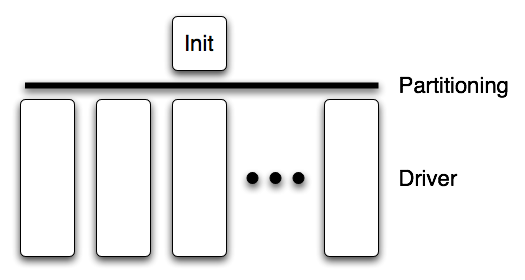
\includegraphics[height=3in]{fig/parfum_structure}
\end{center}
\caption{A typical ParFUM program consists of an {\tt init()} function running in serial context and a {\tt driver()} function running in parallel context.}
\label{fig:parfum_structure}
\end{figure}

In pseudocode, a simple ParFUM program would have the following structure:

\begin{alltt}
     subroutine init
          read the serial mesh and configuration data
     end subroutine
/* after init, the FEM framework partitions the mesh */
     subroutine driver
          get local mesh chunk
          time loop
               FEM computations
               communicate boundary conditions
               more FEM computations
          end time loop
     end subroutine
\end{alltt}

\subsection{ParFUM Programs without init/driver}

Although ParFUM provides the init/driver structure as a convenience to the programmer, you can write a ParFUM program without using init or driver. This is a more flexible approach, but it is more complicated than an init/driver program.

In pseudocode, a ParFUM program with a stand-alone main function might look like this:

\begin{alltt}
   main program
      MPI_Init
      FEM_Init(MPI_COMM_WORLD)
      if (I am master processor)
         read mesh
      partition mesh
      time loop
          FEM computations
          communicate boundary conditions
          more FEM computations
      end time loop
   end main program
\end{alltt}


In this mode, the FEM framework does not set a default reading or writing mesh, and does no partitioning; you must use the FEM\_Mesh routines to create and 
partition your mesh. See the AMPI manual for details on how to declare
the main routine, or the file main.C in ParFUM for an example of how to write a stand-alone main routine. Compiling a ParFUM program without init or driver requires slightly different link flags than a typical ParFUM program, see the compilation section for details.


\subsection{Compilation}

To compile and link a ParFUM program, you must first have a working copy of \charmpp\ and the ParFUM libraries. The process for downloading and building this software is described in section \ref{sec:getting_parfum}.

To compile a FEM program, compile and link using {\tt charmc}, and pass the flag {\tt -language ParFUM}} to charmc when linking. If your program uses its own {\tt main} function rather than init and driver, pass {\tt -language AMPI} instead.

\subsection{Execution}

At runtime, a Charm++/FEM framework program accepts the following
options, in addition to all the usual Charm++ options described in 
the Charm++ ``Installation and Usage Manual''.

\begin{itemize}

\item {\tt +vp} $v$  

Create $v$ mesh chunks, or ``virtual processors''.
By default, the number of mesh chunks is equal to the number of 
physical processors (set with {\tt +p} $p$).


\item {\tt -write}

Skip \kw{driver()}.
After running \kw{init()} normally, the framework partitions the mesh, 
writes the mesh partitions to files, and exits.  As usual, the
{\tt +vp} $v$ option controls the number of mesh partitions.

This option is only used in programs with an {\tt init} function.

\item {\tt -read}

Skip \kw{init()}.
The framework reads the partitioned input mesh from files
and calls \kw{driver()}.  Together with {\tt -write}, this option
allows you to separate out the mesh preparation and partitioning 
phase from the actual parallel solution run.

This can be useful, for example, if \kw{init()} requires more memory 
to hold the unpartitioned mesh than is available on one processor of 
the parallel machine.  To avoid this limitation, you can run the program
with {\tt -write} on a machine with a lot of memory to prepare the input
files, then copy the files and run with {\tt -read} on a machine with 
a lot of processors.

{\tt -read} can also be useful during debugging or performance tuning, 
by skipping the (potentially slow) mesh preparation phase.
This option is only used in programs with a {\tt driver} function.

\item {\tt +tcharm\_trace fem}

Give a diagnostic printout on every call into the ParFUM framework.
This can be useful for locating a sudden crash, or understanding
how the program and framework interact.  Because printing the 
diagnostics can slow a program down, use this option with care.

\end{itemize}
\section{Configuring \pose{}}

\pose{} can be configured in two different ways.  Fundamental
behaviors are controlled by altering values in the {\tt
pose\_config.h} file in the \pose{} installation, and rebuilding
\pose{}.  Many of these configuration options can (and should) be
controlled by command line options.  These will be designated here by
an asterisk ($*$).  See section~\ref{sec:posecommand} for the command line
options.  

\begin{itemize}
\item {\tt {\bf POSE\_STATS\_ON $*$}}\\
	$\circ$ Turn on timing and statistics gathering for internal \pose{}
	operations.  Produces a small slowdown in program.\\
\item {\tt {\bf POSE\_DOP\_ON $*$}}\\
	$\circ$ Turn on timing and statistics gathering for degree of parallelism calculations.  Generates log files that can be loaded by ploticus scripts to produce graphs plotting active entities over time.  Slows down program dramatically.\\
\item {\tt {\bf POSE\_COMM\_ON}}\\
	$\circ$ Turn on streaming communication optimization for small message packing.\\
\item {\tt {\bf COMM\_TIMEOUT}}\\
	$\circ$ Used by streaming communication library. Time to wait (in ?) before sending buffered messages.\\
\item {\tt {\bf COMM\_MAXMSG}}\\
	$\circ$ Used by streaming communication library.  Number of messages to buffer before packing and sending as one.\\
\item {\tt {\bf LB\_ON $*$}}\\
	$\circ$ Turn on \pose{} load balancing.\\
\item {\tt {\bf STORE\_RATE $*$}}\\
	$\circ$ Default checkpointing rate: 1 for every {\tt STORE\_RATE} events.\\
\item {\tt {\bf SPEC\_WINDOW $*$}}\\
	$\circ$ Speculative window size: this is how far (in virtual time units) ahead of GVT posers are allowed to go.\\
\item {\tt {\bf MIN\_LEASH $*$}} and {\tt {\bf MAX\_LEASH $*$}}\\
	$\circ$ Bounds on the speculative window, these are adjusted by adaptive synchronization strategies.\\
\item {\tt {\bf LEASH\_FLEX $*$}}\\
	$\circ$ Granularity of flexibility when speculative window is shrunk or expanded.\\
\item {\tt {\bf MAX\_POOL\_SIZE}}\\
	$\circ$ Memory used by event messages is recycled.  This controls how many messages of a particular size will be kept on hand.
\item {\tt {\bf MAX\_RECYCLABLE}}\\
	$\circ$ This is the largest size of message that will be recycled.
\item {\tt {\bf LB\_SKIP $*$}}\\
	$\circ$ This controls the frequency of load balance invocation.  1 in every {\tt LB\_SKIP} executions of the GVT algorithm will invoke load balancing.
\item {\tt {\bf LB\_THRESHOLD $*$}}\\
	$\circ$ What the heck does this number mean?  I can't remember.  I'll have to look through the code... later.  Meanwhile, I think this indicates some sort of threshold a single processor has to cross before we even bother with analyzing the load.\\
\item {\tt {\bf LB\_DIFF $*$}}\\
	$\circ$ Once the load has been analyzed, we compute the difference between the max and min PE loads.  Only if this difference exceeds {\tt LB\_DIFF} do we bother migrating posers.\\
\end{itemize}

Several of the above flags and constants will be eliminated as the adaptive strategy is expanded.  What remains will eventually become run-time options.

\subsection{\pose{} Command Line Options}
\label{sec:posecommand}

Command line options are handled like \charmpp{} command line
parameters.  For namespace purity all \pose{} command line options
have a \_pose suffix.  They can be inspected by appending a -h to an
execution of a \pose{} program.  Command line options override any
defaults set in the {\tt pose\_config.h} file

\begin{itemize}
\item {\tt {\bf +stats\_pose}}\\
	$\circ$ Turn on timing and statistics gathering for internal \pose{}
	operations.  Produces a small slowdown in program.\\
\item {\tt {\bf +dop\_pose}}\\
	$\circ$ Turn on timing and statistics gathering for degree of parallelism calculations.  Generates log files that can be loaded by ploticus scripts to produce graphs plotting active entities over time.  Slows down program dramatically.\\
\item {\tt {\bf +lb\_on\_pose}}\\
	$\circ$ Turn on \pose{} load balancing.\\
\item {\tt {\bf +store\_rate\_pose N}}\\
	$\circ$ Default checkpointing rate: 1 for every {\tt STORE\_RATE} events.\\
\item {\tt {\bf +spec\_window\_pose N}}\\
	$\circ$ Speculative window size: this is how far (in virtual time units) ahead of GVT posers are allowed to go.\\
\item {\tt {\bf +min\_leash\_pose N}} and {\tt {\bf +min\_leash\_pose N}}\\
	$\circ$ Bounds on the speculative window, these are adjusted by adaptive synchronization strategies.\\
\item {\tt {\bf +leash\_flex\_pose N}}\\
	$\circ$ Granularity of flexibility when speculative window is shrunk or expanded.\\
\item {\tt {\bf +lb\_skip\_pose N}}\\
	$\circ$ This controls the frequency of load balance invocation.  1 in every {\tt LB\_SKIP} executions of the GVT algorithm will invoke load balancing.
\item {\tt {\bf +lb\_threshold\_pose N}}\\
	$\circ$ Minimum threshold for load balancing, default is 4000
\item {\tt {\bf +lb\_diff\_pose N}}\\
	$\circ$ Once the load has been analyzed, we compute the difference between the max and min PE loads.  Only if this difference exceeds {\tt LB\_DIFF} do we bother migrating posers.\\
\item {\tt {\bf +checkpoint\_gvt\_pose N}}\\
	$\circ$ Checkpoint to disk approximately every N GVT ticks (N is an integer).  The default is 0, which indicates no checkpointing.
\item {\tt {\bf +checkpoint\_time\_pose N}}\\
	$\circ$ Checkpoint to disk every N seconds (N is an integer).  The default is 0, which indicates no checkpointing.  If both this parameter and +checkpoint\_gvt\_pose are greater than 0, a warning will be given, the value of this parameter will be set to 0, and POSE will checkpoint based on GVT ticks.
\end{itemize}

As a technical point, pose command line parsing is done inside the
{\tt POSE\_init()} call.  Therefore, the most consistent behavior for
interleaving pose command line options with user application options
will be achieved by calling {\tt POSE\_init()} before handling user
application command line arguments.  

\section{Communication Optimizations}
\section{Load Balancing}
\section{Glossary of \pose{}-specific Terms}

\begin{itemize}
\item {\tt void {\bf POSE\_init}()}\\
	$\circ$ Initializes various items in \pose{}; creates the load balancer
	if load balancing is turned on; initializes the statistics
	gathering facility if statistics are turned on.\\
	$\circ$ Must be called in user's main program prior to creation of any
	simulation objects or reference to any other \pose{} construct.
\item {\tt void {\bf POSE\_start}()}\\
	$\circ$ Sets busy wait to default if none specified; starts
	quiescence detection; starts simulation timer.\\
	$\circ$ Must be called in user's main program when simulation
	should start.
\item {\tt void {\bf POSE\_registerCallBack}(CkCallback cb)}\\
	$\circ$ Registers callback function with \pose{} -- when program
	ends or quiesces, function is called.\\
	$\circ$ CkCallback is created with the index of the callback
	function and a proxy to the object that function is to be
	called on.  For example, to register the function {\tt wrapUp}
	in the main module as a callback:

\begin{verbatim}
  CProxy_main M(mainhandle);
  POSE_registerCallBack(CkCallback(CkIndex_main::wrapUp(), M));
\end{verbatim}

\item {\tt void {\bf POSE\_stop}()}\\
	$\circ$ Commits remaining events; prints final time and
	statistics (if on); calls callback function.\\
	$\circ$ Called internally when quiescence is detected or
	program reaches {\tt POSE\_endtime}.
\item {\tt void {\bf POSE\_exit}()}\\
	$\circ$ Similar to {\tt CkExit()}.
\item {\tt void {\bf POSE\_set\_busy\_wait}(int n)}\\
	$\circ$ Used to control granularity of events; when calling
	{\tt POSE\_busy\_wait}, program busywaits for time to compute $fib(n)$.
\item {\tt void {\bf POSE\_busy\_wait}()}\\
	$\circ$ Busywait for time to compute $fib(n)$ where n is either
	1 or set by {\tt POSE\_set\_busy\_wait}.
\item {\tt {\bf POSE\_useET(t)}}\\
	$\circ$ Set program to terminate when global
	virtual time (GVT) reaches $t$.
\item {\tt {\bf POSE\_useID()}}\\
	$\circ$ Set program to terminate when no events are available
	in the simulation.
\item {\tt void {\bf POSE\_create}({\it constructorName}(eventMsg *m), int
handle, int atTime)}\\
	$\circ$ Creates a poser object given its constructor, an event
	message $m$ of the appropriate type, any integer as the handle
	(by which the object will be referred from then on), and a
	time (in simulation timesteps) at which it should be created.\\ 
	$\circ$ The handle can be thought of as a chare array element
	index in Charm++.
\item {\tt void {\bf POSE\_invoke\_at}({\it methodName}(eventMsg *m),
{\it className}, int handle, int atTime)}\\
	$\circ$ Send a {\it methodName} event with message $m$ to an
	object of type {\it className} designated by handle $handle$
	at time specified by $atTime$.\\
	$\circ$ This can be used by non-poser objects in the \pose{}
	module to inject events into the system being simulated.  It
	should not be used by a poser object to generate an event.
\item {\tt void {\bf POSE\_invoke}({\it methodName}(eventMsg *m),
{\it className}, int handle, int timeOffset)}\\
	$\circ$ Send a {\it methodName} event with message $m$ to an
	object of type {\it className} designated by handle $handle$
	at current OVT + $timeOffset$.\\
	$\circ$ This is used by poser objects to send events from one
	poser to another.
\item {\tt void {\bf POSE\_local\_invoke}({\it methodName}(eventMsg
	*m), int timeOffset)}\\
	$\circ$ Send a {\it methodName} event with message $m$ to this
	object at current OVT + $timeOffset$.\\
	$\circ$ This is used by poser objects to send events to themselves.
\item {\tt void {\bf CommitPrintf}(char *s, args...)}\\
	$\circ$ Buffered print statement; prints when event is
	committed (i.e. will not be rolled back).\\
	$\circ$ Currently, must be called on the wrapper class
	(parent) to work properly, but a fix for this is in the works.
\item {\tt void {\bf CommitError}(char *s, args...)}\\
	$\circ$ Buffered error statement; prints and aborts program
	when event is committed.\\
	$\circ$ Currently, must be called on the wrapper class
	(parent) to work properly, but a fix for this is in the works.
\item {\tt void {\bf elapse}(int n)}\\
	$\circ$ Elapse $n$ simulation time units.
\item {\tt {\bf poser}}\\
	$\circ$ Keyword (used in place of chare) to denote a poser
	object in the {\tt .ci} file of a \pose{} module.
\item {\tt {\bf event}}\\
	$\circ$ Keyword used in square brackets in the {\tt .ci} file
	of a \pose{} module to denote that the entry method is an event method.
\item {\tt {\bf eventMsg}}\\
	$\circ$ Base class for all event messages; provides timestamp,
	priority and many other properties.
\item {\tt {\bf sim}}\\
	$\circ$ Base class of all wrapper classes.
\item {\tt {\bf strat}}\\
	$\circ$ Base class of all strategy classes.
\item {\tt {\bf con}}\\
	$\circ$ Simple conservative strategy class.
\item {\tt {\bf opt, opt2, opt3, spec, adapt, adapt2}}\\
	$\circ$ Optimistic strategy classes.
\item {\tt {\bf rep}}\\
	$\circ$ Base class for all representation classes.
\item {\tt {\bf chpt}}\\
	$\circ$ Simple checkpointing representation class.
\item {\tt {\bf OVT()}}\\
	$\circ$ Returns the object virtual time (OVT) of the poser in
	which it is called
\item {\tt void $MySim$::{\bf terminus}()}\\
	$\circ$ When simulation has terminated and program is about to exit, this method is called on all posers.  Implemented as an empty method in the base {\tt rep} class, the programmer may choose to override this with whatever actions may need to be performed per object at the end of the simulation.
\end{itemize}


\end{document}
